\chapter{Accepttest of RMS compressor}\label{app:journal_Frequency_Response}
The purpose of this test is verify requirement \textbf{XX} concerning RMS compressor.

\section{Setup}
The setup of this test are depicted in \textbf{XX}, where the equipment is catalogued in \textbf{XX}, and described as follows:

\begin{itemize}
\item Frequency reponse will be measured by a Harmonie analyzer.
\item A noise generator will generate the following for the test. 
\begin{itemize}
\item Sampling frequency: 48000 Hz.
\item Generator amplitude: \textbf{X} V.
\item Pink noise.
\end{itemize}
\item The software of the system used for the bypass test is found at CD. \todo[inline]{CD}
\item The software of the system used for the stage1 test is found at CD. \todo[inline]{CD}
\item The software of the system used for the full system test is found at CD. \todo[inline]{CD}
\end{itemize}


\subsection*{Test Setup}
\begin{figure}[H]
\centering
\includegraphics[width=0.9\textwidth]{FreqReponseSetup.png}
\label{fig:AcceptFreqResponse}
\caption{Test setup.}
\end{figure}

\subsection*{Equipment used and AAU-no.}

\begin{table}[H]
\centering
\ra{1.3}
\begin{tabular}{S[table-format=1]ccc} \toprule
    {Item} & {Description} & {AAU-no} \\ \bottomrule 
    1      &  Harmonie  & 60923  \\ 
    2      &  Harmonie PC  & 56524  \\ 
    3      &  Sine/Noise generator type 1049  & 08233  \\  \bottomrule 
\end{tabular}
\caption{Table over equipment used in the test}
\label{tab:UsedEquipmentFreqResponse}
\end{table}
\vspace{-5mm}


\section{Procedure}
The procedure for this experiment is described as follows:
\vspace{-5mm}
\begin{enumerate}
\item Setup the noise generator with the mentioned settings.
\item Setup the Harmonie and the Harmonie PC
\item Start recording on the PC
\item When finished save the results of the test.
\end{enumerate}

\section{Data Extraction}
The raw dat for the Bypass can be found at the CD \todo[inline]{CD}
The raw dat for the Full system can be found at the CD \todo[inline]{CD}
There are 30 bands from 20 Hz to 20 kHz, see \autoref{tb:freqBandsAppendix}, where a magnitude is given in dB for each band. 10 different measurements have been taken for both bypass and the full system. The mean and standard deviation (std) have been found for each band as has been plotted. The two bands 25 Hz and 20000 Hz has been removed from the plots because of large deviation and therefore not deemed usefull.

\begin{table}[H]
\centering
\begin{tabular}{|c|c|c|c|c|c|c|c|c|c|}
\hline
\multicolumn{10}{|c|}{Bands [Hz]}                                       \\ \hline
25   & 31.5 & 40   & 50   & 63   & 80   & 100   & 125   & 160   & 200   \\ \hline
250  & 315  & 400  & 500  & 630  & 800  & 1000  & 1250  & 1600  & 2000  \\ \hline
2500 & 3150 & 4000 & 5000 & 6300 & 8000 & 10000 & 12500 & 16000 & 20000 \\ \hline
\end{tabular}
\caption{Frequency bands.}
\label{tb:freqBandsAppendix}
\end{table}

\section{Analysis}

\begin{figure}[H]
	\centering
	\tikzsetnextfilename{FreqNoiseComp}
	% This file was created by matlab2tikz.
%
%The latest updates can be retrieved from
%  http://www.mathworks.com/matlabcentral/fileexchange/22022-matlab2tikz-matlab2tikz
%where you can also make suggestions and rate matlab2tikz.
%
\definecolor{mycolor1}{rgb}{0.00000,0.44700,0.74100}%
\definecolor{mycolor2}{rgb}{0.85000,0.32500,0.09800}%
%
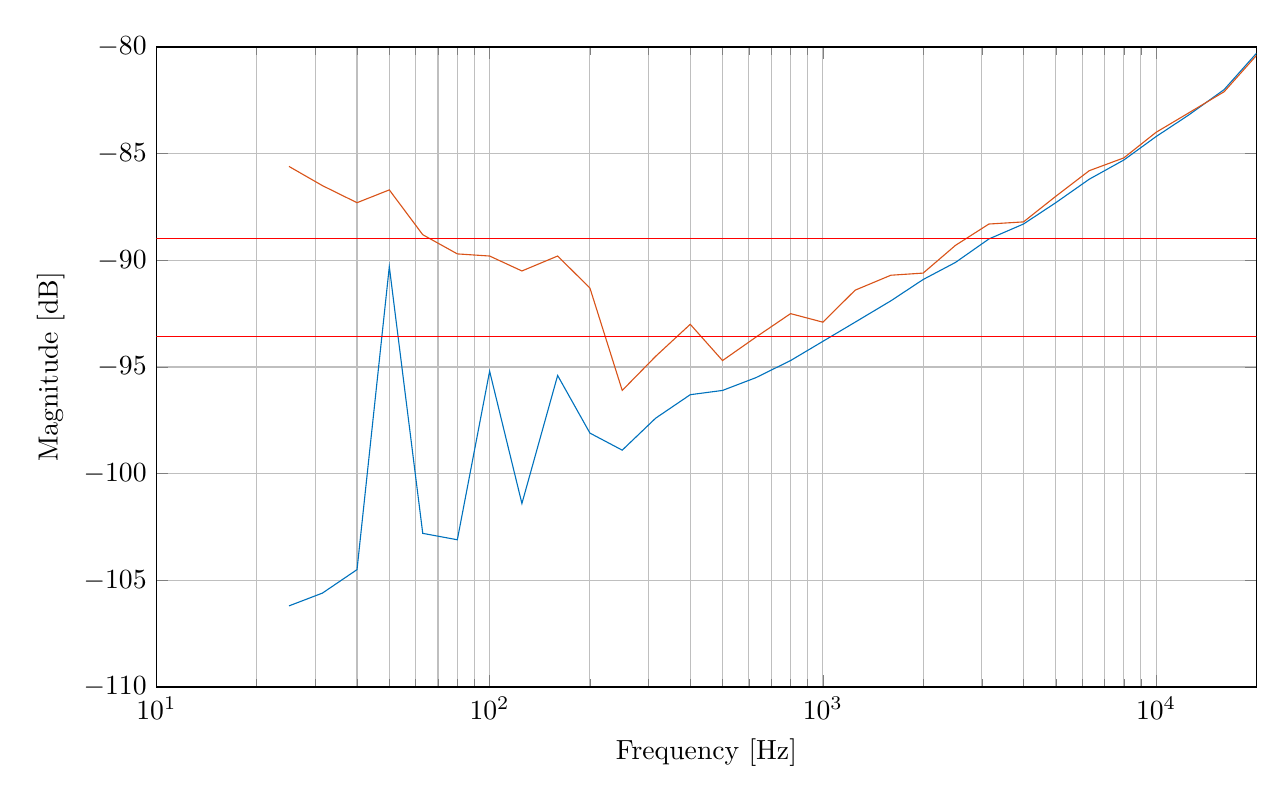
\begin{tikzpicture}

\begin{axis}[%
width=5.5in,
height=3.2in,
at={(0.758in,0.481in)},
scale only axis,
xmode=log,
xmin=10,
xmax=20000,
xminorticks=true,
xlabel={Frequency [Hz]},
xmajorgrids,
xminorgrids,
ymin=-110,
ymax=-80,
ylabel={Magnitude [dB]},
ymajorgrids,
axis background/.style={fill=white}
]
\addplot [color=mycolor1,solid,forget plot]
  table[row sep=crcr]{%
25	-106.2\\
31.5	-105.6\\
40	-104.5\\
50	-90.3\\
63	-102.8\\
80	-103.1\\
100	-95.2\\
125	-101.4\\
160	-95.4\\
200	-98.1\\
250	-98.9\\
315	-97.4\\
400	-96.3\\
500	-96.1\\
630	-95.5\\
800	-94.7\\
1000	-93.8\\
1250	-92.9\\
1600	-91.9\\
2000	-90.9\\
2500	-90.1\\
3150	-89\\
4000	-88.3\\
5000	-87.3\\
6300	-86.2\\
8000	-85.3\\
10000	-84.2\\
12500	-83.2\\
16000	-82\\
20000	-80.3\\
};
\addplot [color=mycolor2,solid,forget plot]
  table[row sep=crcr]{%
25	-85.6\\
31.5	-86.5\\
40	-87.3\\
50	-86.7\\
63	-88.8\\
80	-89.7\\
100	-89.8\\
125	-90.5\\
160	-89.8\\
200	-91.3\\
250	-96.1\\
315	-94.5\\
400	-93\\
500	-94.7\\
630	-93.6\\
800	-92.5\\
1000	-92.9\\
1250	-91.4\\
1600	-90.7\\
2000	-90.6\\
2500	-89.3\\
3150	-88.3\\
4000	-88.2\\
5000	-87\\
6300	-85.8\\
8000	-85.2\\
10000	-84\\
12500	-83.1\\
16000	-82.1\\
20000	-80.4\\
};
\addplot [color=red,solid,forget plot]
  table[row sep=crcr]{%
10	-93.5633333333333\\
100000	-93.5633333333333\\
};
\addplot [color=red,solid,forget plot]
  table[row sep=crcr]{%
10	-88.98\\
100000	-88.98\\
};
\end{axis}
\end{tikzpicture}%
	\caption{Frequency reposnse of bypassed noisefloow (blue) and full system noise floor (orange). Mean bypass=-93.5633, Mean system=-88.98.}
	\label{fig:FFreqNoiseComp}
\end{figure}


\section{Error sources}


\section{Conclusion}
From the test of bypass and fulle system it can be concluded that 